%% This is an example first chapter.  You should put chapter/appendix that you
%% write into a separate file, and add a line \include{yourfilename} to
%% main.tex, where `yourfilename.tex' is the name of the chapter/appendix file.
%% You can process specific files by typing their names in at the 
%% \files=
%% prompt when you run the file main.tex through LaTeX.

\singlespacing{

   \textbf{Purpose/Suitability/Motivation:}\\
        What is the PROBLEM? Why is it IMPORTANT?\\
        How might the thesis results be used? What might it lead toward?\\
        What is the potential impact of the work? \\
   \textbf{Description/Approach:}\\
        What are you proposing to build or develop?\\
        What technologies will you use and are they available or will you develop them from scratch?\\
        What resources are required and are these available?\\
        What are the limits of what you will address? \\
    \textbf{Originality/Contribution:}\\
        What else has been done in this area of research?\\
        What is the state of the art?\\
        What other approaches have been taken and how are they different from your approach?\\
        What are the original contributions of your work to the field? \\
    \textbf{Evaluation/Scope:}\\
        How will you evaluate your work?\\
        How will you know you are done?\\
        What do you expect to accomplish/prove? \\


\chapter{Introduction}

The current research goals of CBA center around a new method of 


\section{Digital Assembly}

The discrete 

\subsection{Macro Assembly}

Cheung showed that carbon fiber composite parts can be reversibly assembled to form ultralight materials \cite{Cheung2013}.  This work demonstrated programmable flexibility in the structures by pattering rigid and flexural elements across an assembly.  Additional research into digital assembly of structural elements is ongoing at CBA, including modeling of the parts and assemblies using finite element analysis\cite{Calisch2014} and designing new part geometries and robotic assemblers\cite{Carney2015}.

\subsection{Micro Assembly}

%\begin{figure}
%  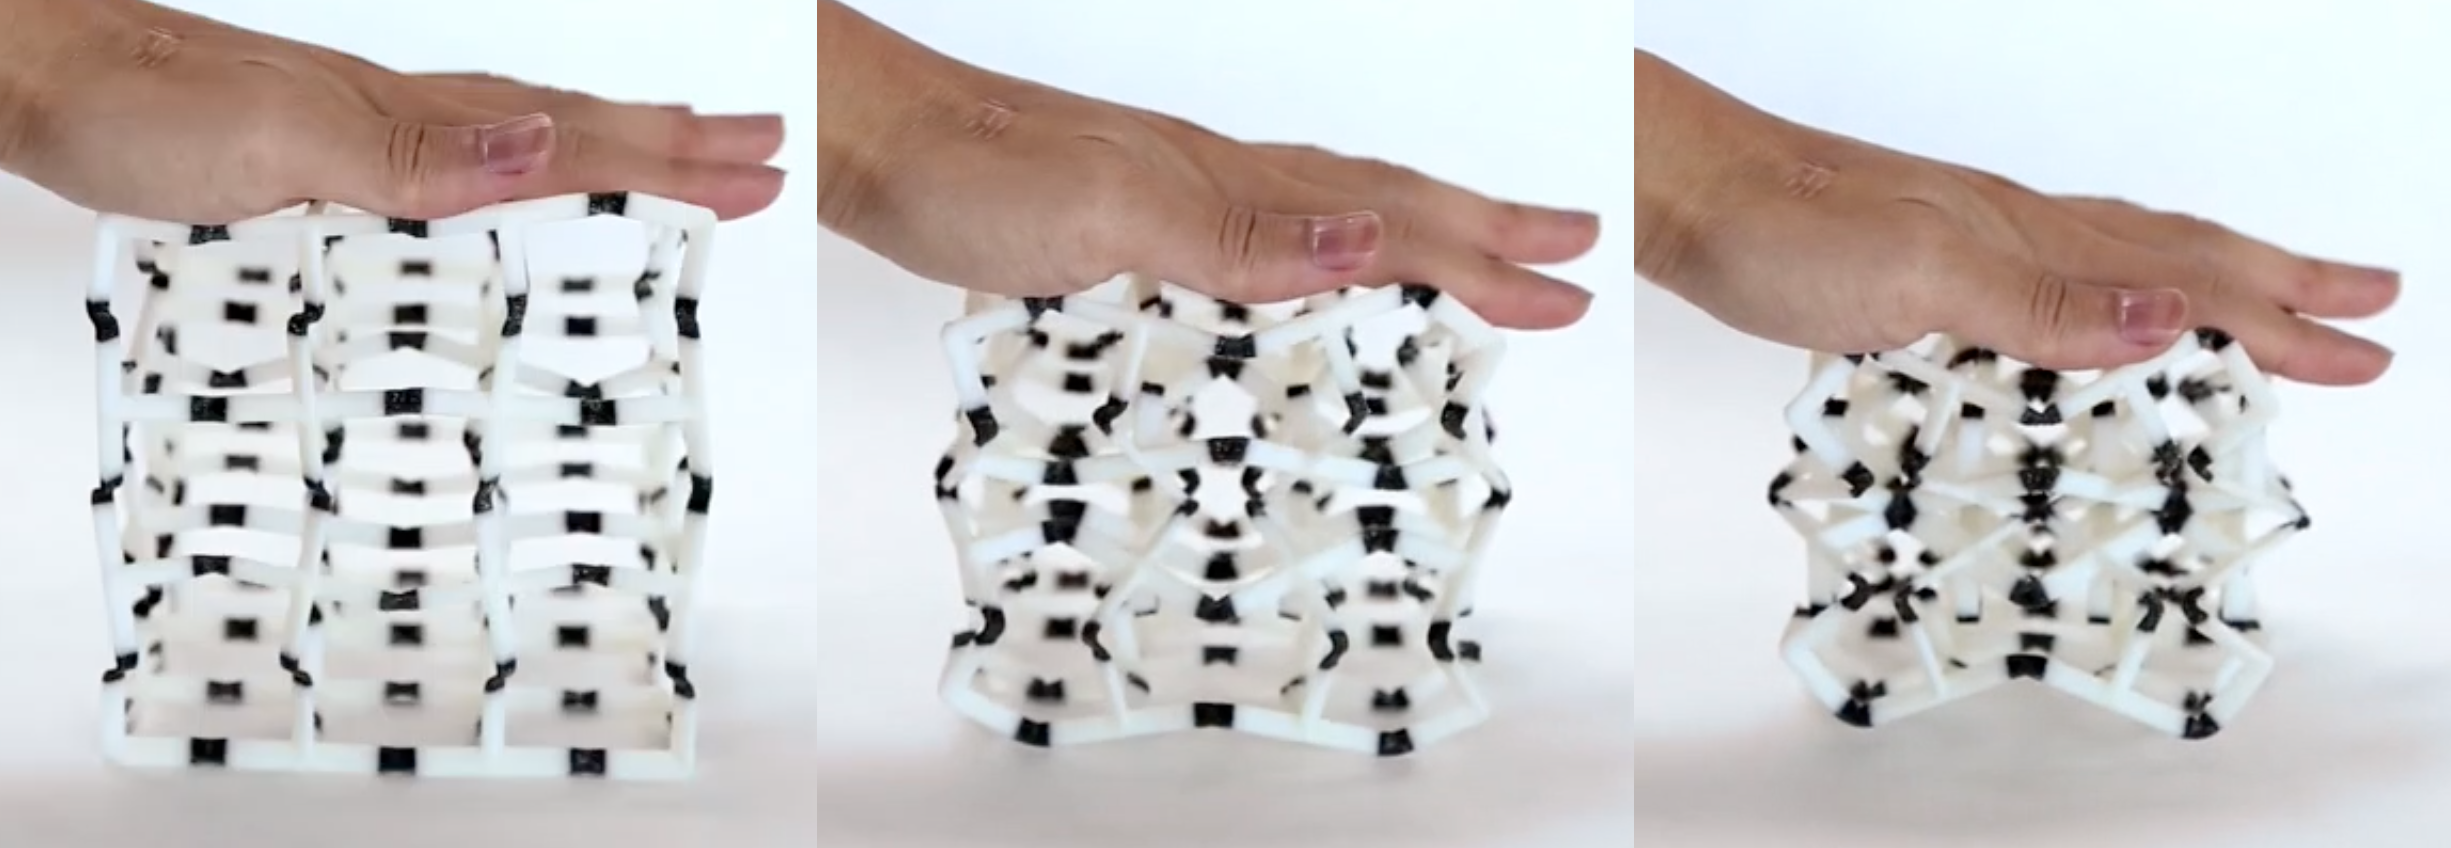
\includegraphics[width=\linewidth]{objetMultimaterial.png}
%  \caption{Mechanical properties programmed by material deposition in Objet 3D print.}
%  \label{fig: objetMultimaterial}
%\end{figure}

Will - look at will's thesis to find other examples of discrete micro assembly \cite{Langford2014}.
\\

Though not a reversible process, multimaterial 3D printing (most notably by the Objet printer) deposits material in voxels on the order of ~10$\mu$M$^{3}$ with a total build volume on the order of 1x10$^{10}$ voxels \cite{Objet1000}.  Multimaterial 3d printing has been demonstrated in optical \cite{Willis2012}, electronic \cite{Ahn2009}, and structural applications \cite{Skouras2013} \cite{Schumacher}, and other physical optimizations of objects \cite{Bacher2014}.

\subsection{Nano Assembly}

DNA bricks is a system of discrete assembly based on complementary base pair interactions of short segments of DNA\cite{Ke2012}; DNA bricks is a branch of a  field called DNA origami\cite{Rothemund2006} or DNA computing.  The brick assemblies have a spatial resolution of 2.5nm and the longest dimension of a DNA brick assembly measures on the order of 1$\mu$M\cite{Ke2014}.
\\

Biology gives an example of discrete construction capable of producing a wide variety of morphologies and functions.  Using just 20 amino acids, a cell is able to form proteins with an immense variety of morphologies and functions to carry out the tasks of life.  Though it's not an engineered system and it doesn't adhere to a strict lattice configuration, biology serves as a demonstration of the possibilities of discrete construction.
\\

An active area of synthetic biology explores the possibility of creating a viable cell from scratch based on knowledge about the core systems required for metabolism, cell maintainance, and self replication\cite{Forster2006}.  To date, efforts at creating this "minimal cell" have only been successful using a top down approach - starting with an organism with a minimal genome and reducing its genes further\cite{Glass2006}\cite{Gibson2010}.

\section{Related CAD and Simulation Tools}

Design in a discrete 

%\begin{figure}
%  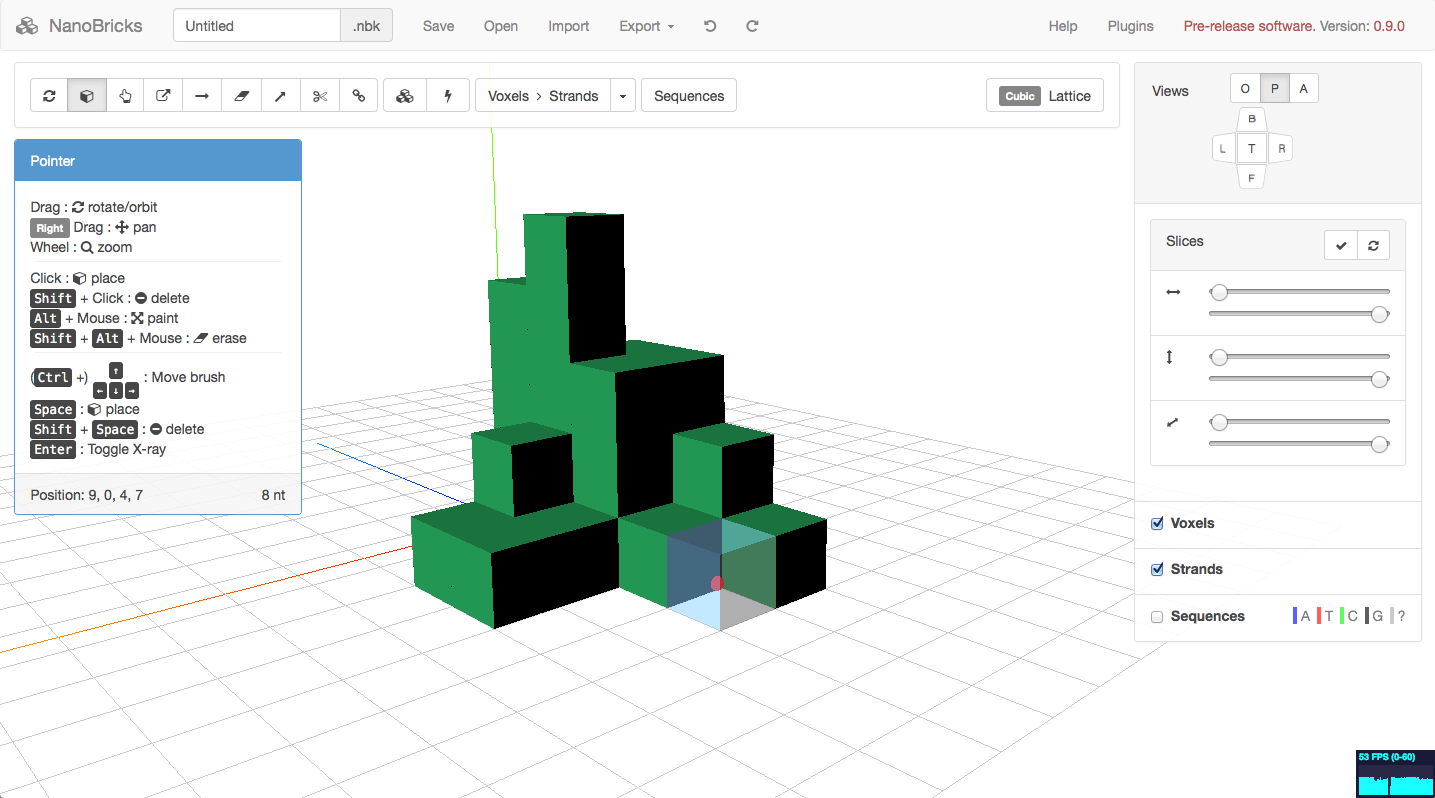
\includegraphics[width=\linewidth]{nanoBricks.png}
%  \caption{Screenshot of NanoBricks, a voxel-based design tool for DNA Bricks by the Peng Yin Lab.}
%  \label{fig:nanoBricks}
%\end{figure}
%Peng Yin's lab at Harvard recently released a beta version of \href{http://yin.hms.harvard.edu/bricks/try/}{Nanobricks}, their own voxel-based design tool for DNA Bricks (Fig~\ref{fig:nanoBricks}).  Nanobricks allows a user to design with voxels on a cubic lattice either by interacting with a 3D interface, through a scripting API, or importing STL geometry.  Then the voxel-based designs are converted to sequences and exported as a text file; the sequences may be generated randomly or from a predefined library of bricks.  Other lattice types (honeycomb, spline) are in development, but not yet fully supported in Nanobricks.



\begin{figure}
  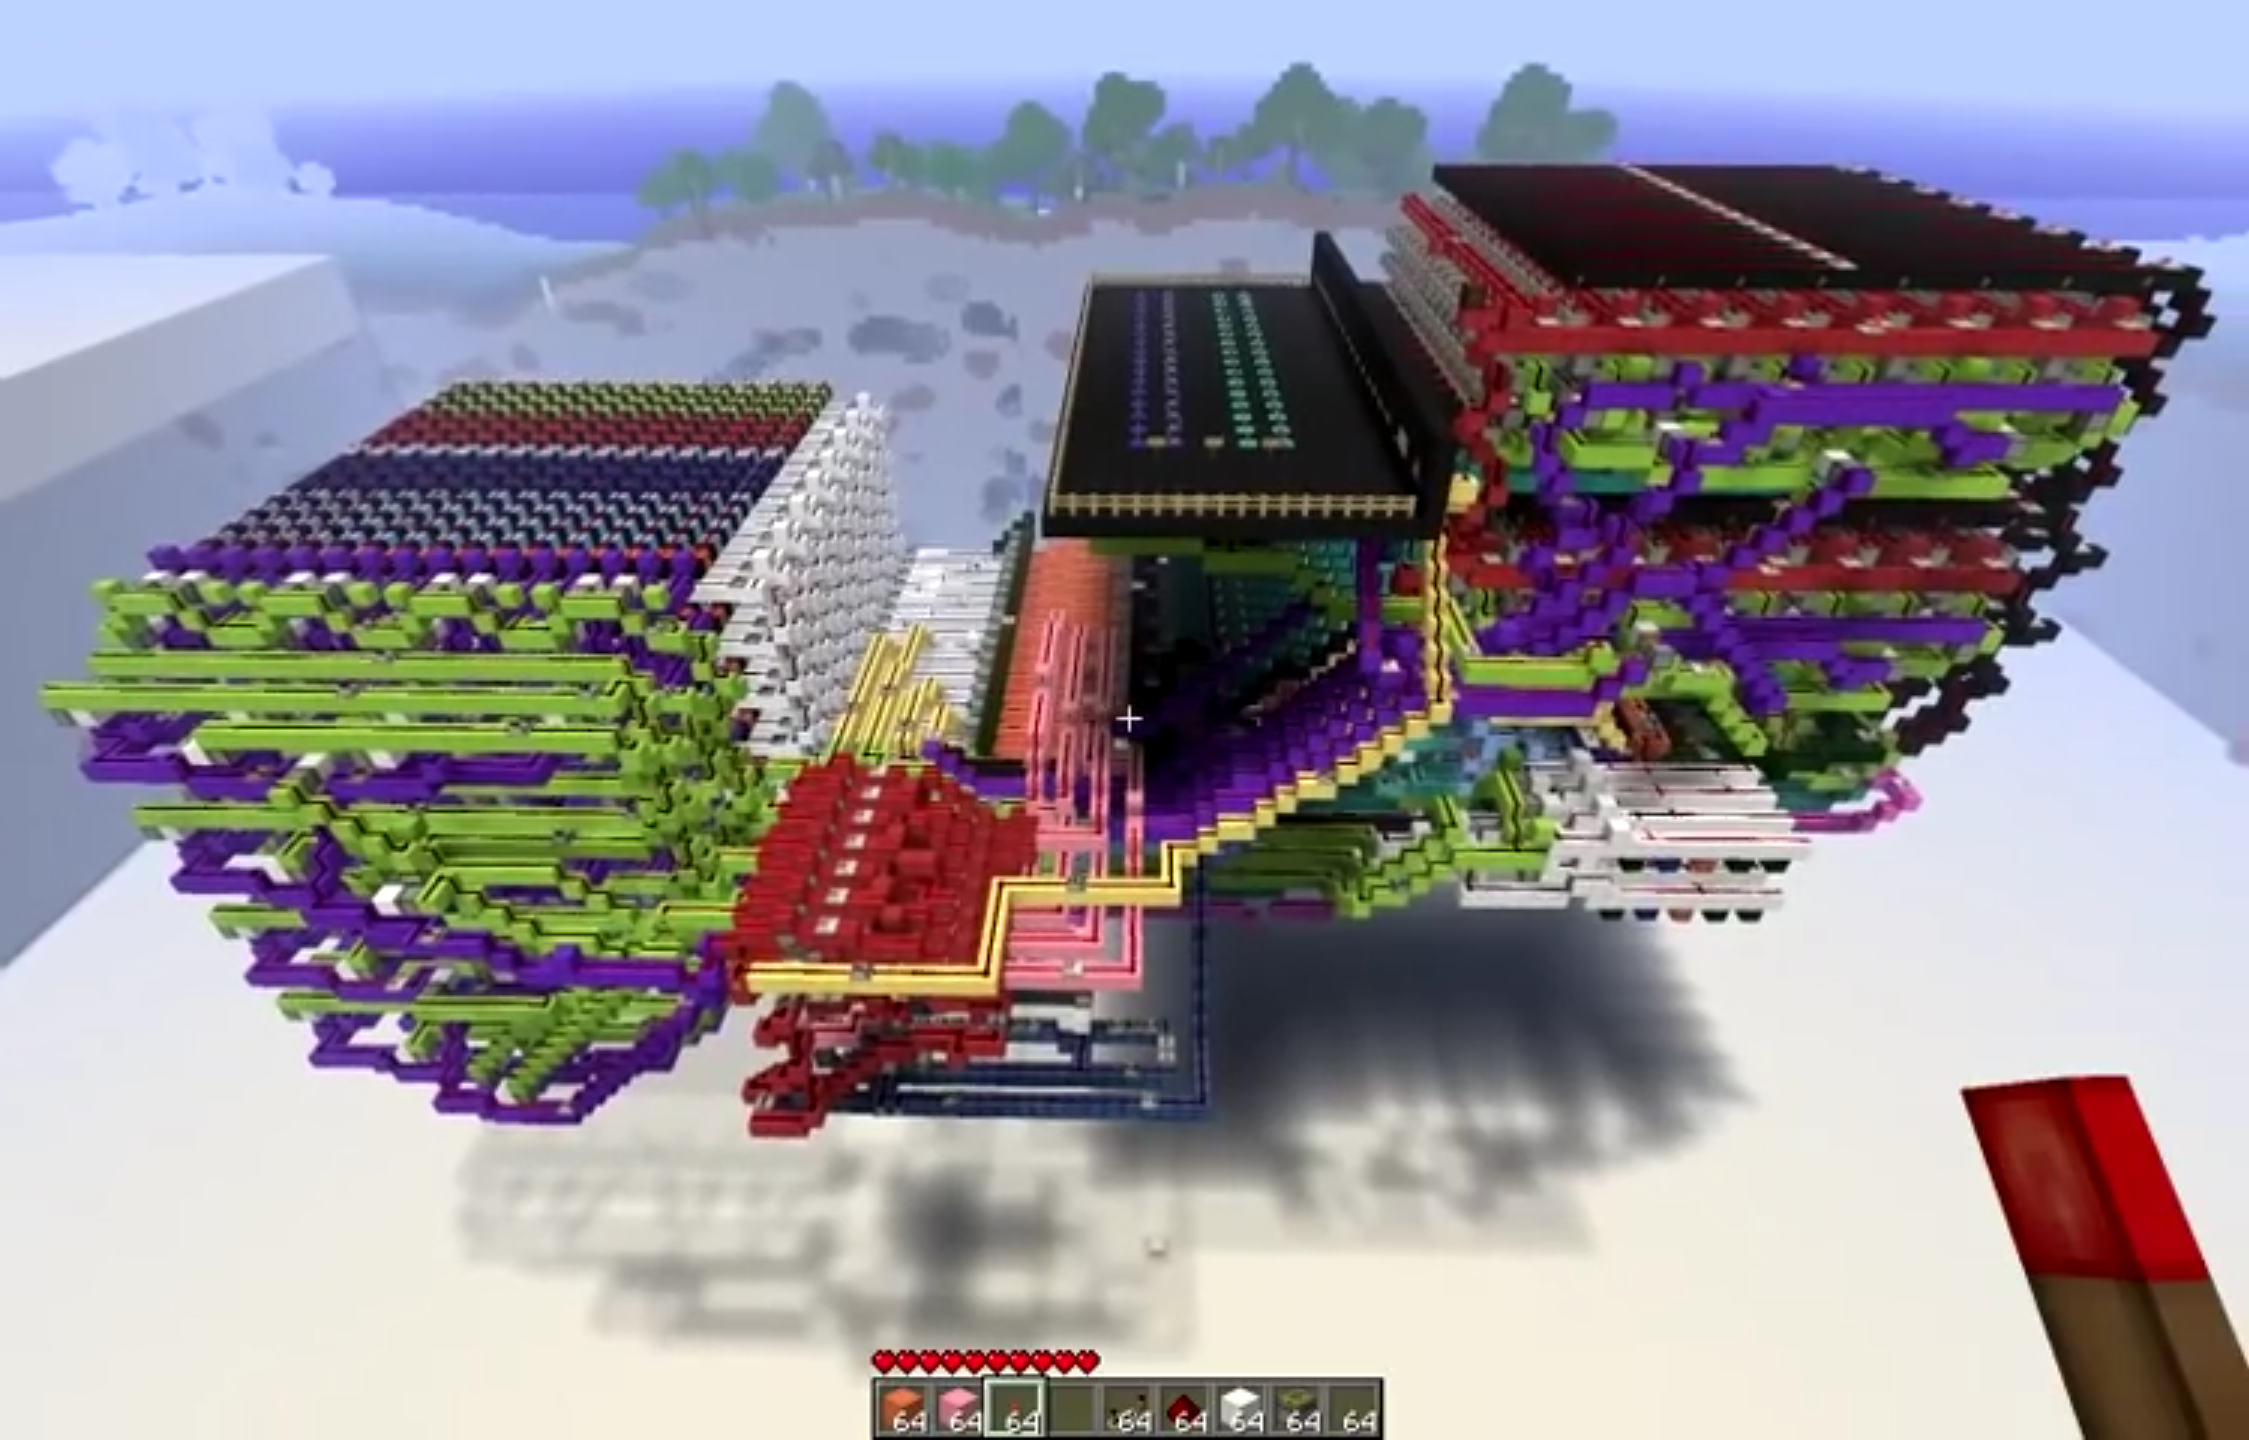
\includegraphics[width=\linewidth]{minecraft.png}
  \caption{Screenshot of a 16 bit computer built in Minecraft by user Ohm.  Full video available on \href{https://www.youtube.com/watch?v=KzrFzkb3A4o}{YouTube}.}
  \label{fig:minecraft}
\end{figure}
Another notable example of voxel-based design is \href{https://minecraft.net/}{Minecraft}, a PC game that give players the ability to construct their own worlds from --- different functional block types.
\\

voxcad\cite{Hiller2014a}
voxel for multi material 3d printing
\\

\href{https://www.youtube.com/watch?feature=player_embedded&v=PBXO_6Jn1fs}{CBlock3D}
\\

\href{http://golly.sourceforge.net/}{Golly} is a 2D cellular automata simulator originally meant for Conway's game of life, but is extendable to other rulesets.  It implements Gosper's Hashlife 
\\

Peng Yin's lab at Harvard recently released a beta version of \href{http://yin.hms.harvard.edu/bricks/try/}{Nanobricks}, a voxel-based design tool for DNA Bricks.  Nanobricks allows a user to design nano-scale structures with voxels on a cubic lattice, and voxel-based designs are converted to sequences and exported as a text file.
\\

\begin{figure}
  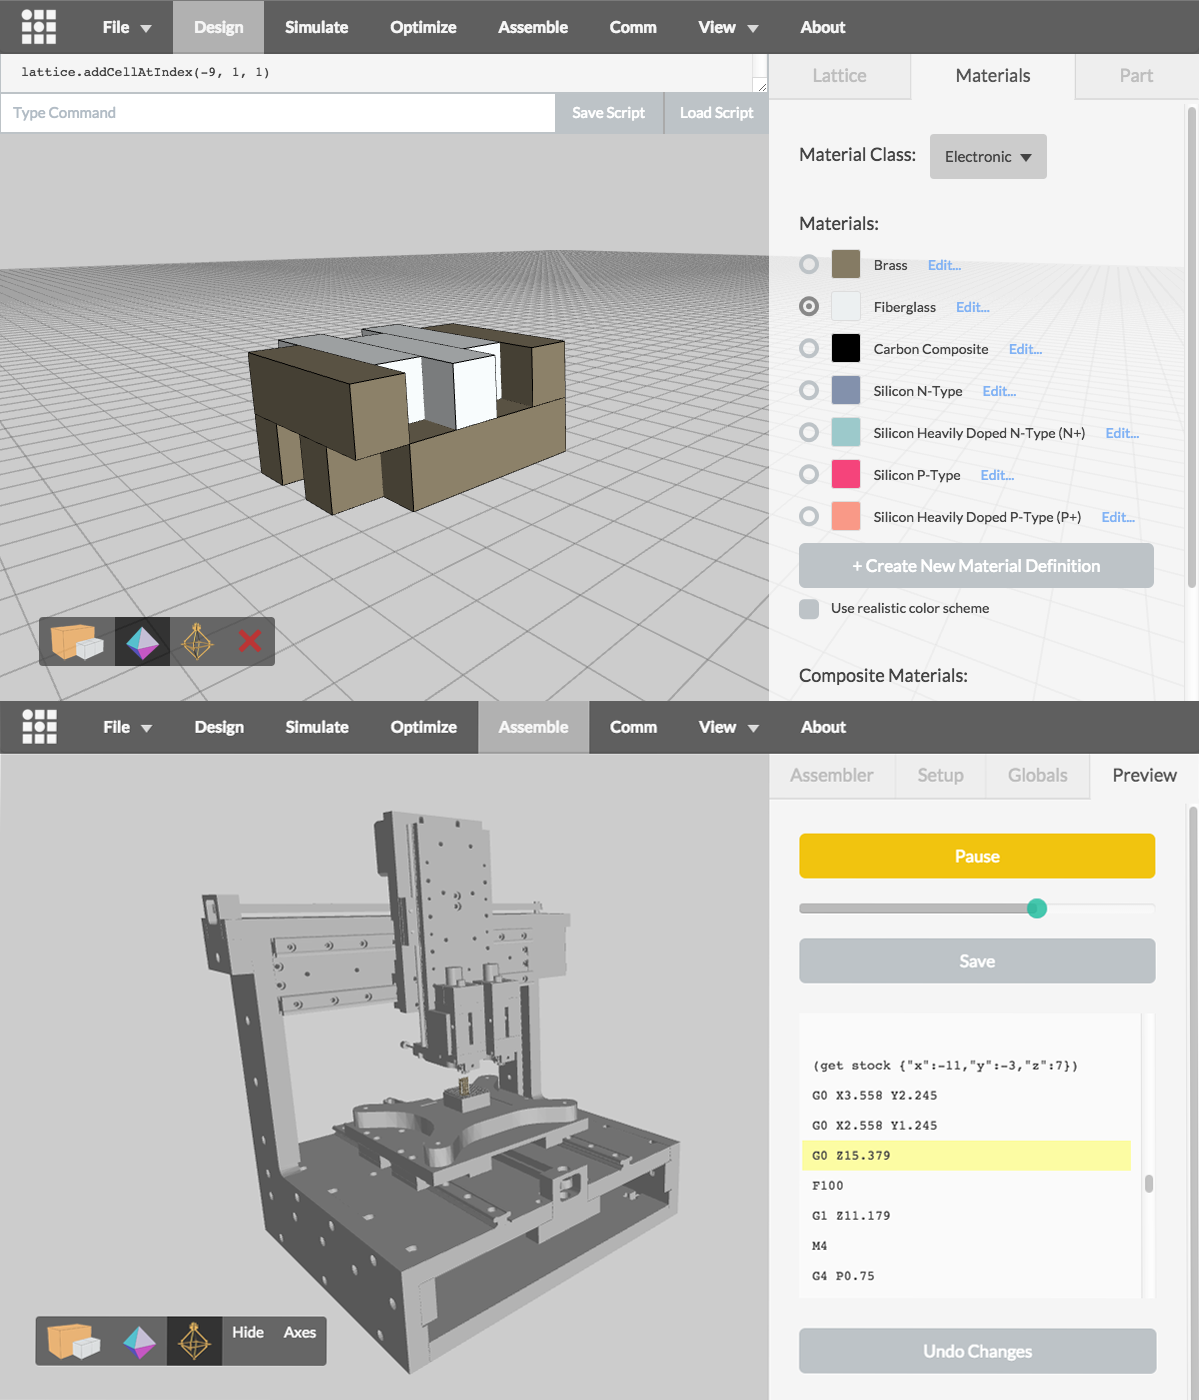
\includegraphics[width=\linewidth]{designAssemblyGUI.png}
  \caption{CAD and CAM GUI of my .}
  \label{fig: designAssemblyGUI}
\end{figure}
\href{http://dma.cba.mit.edu/dmdesign/}{DMDesign} is a CAD/CAM environment for digital materials I've been developing that supports the research efforts into part  and assembler design at CBA.  



\section{Proposed Work}

In Cellular Automata (CA) literature, a machine that can be programmed to build any number of structures, including itself, is called a "universal constructor".  The basic requirements of a universal constructor are well formulated\cite{Neumann1966}, and many implementations exist in various cellular automata worlds (\href{https://www.youtube.com/watch?v=A8B5MbHPlH0}{Conway}, \href{https://en.wikipedia.org/wiki/Von_Neumann_universal_constructor#/media/File:Nobili_Pesavento_2reps.png}{Von Neuman}, \href{https://www.youtube.com/watch?v=PBXO_6Jn1fs}{CBlocks3D}).  However, all of these implementations violate basic physical laws - matter is created or destroyed at will, cells are considered massless, interactions between cells are not modeled.
\\

I propose to build a Design/Simulation environment for digital materials based on real materials and classical physics, so that structures designed within this virtual environment may be physically realized one day.  I will use this vital sandbox to design basic functional elements needed towards the eventual goal of building a physically realizable self-assembling machine.  Some elements of interest include mechanisms for grasping and moving parts in the assembler's environment, locomotion systems, information storage and retrieval, amplification, and digital logic.

\subsection{Design}

\begin{figure}
  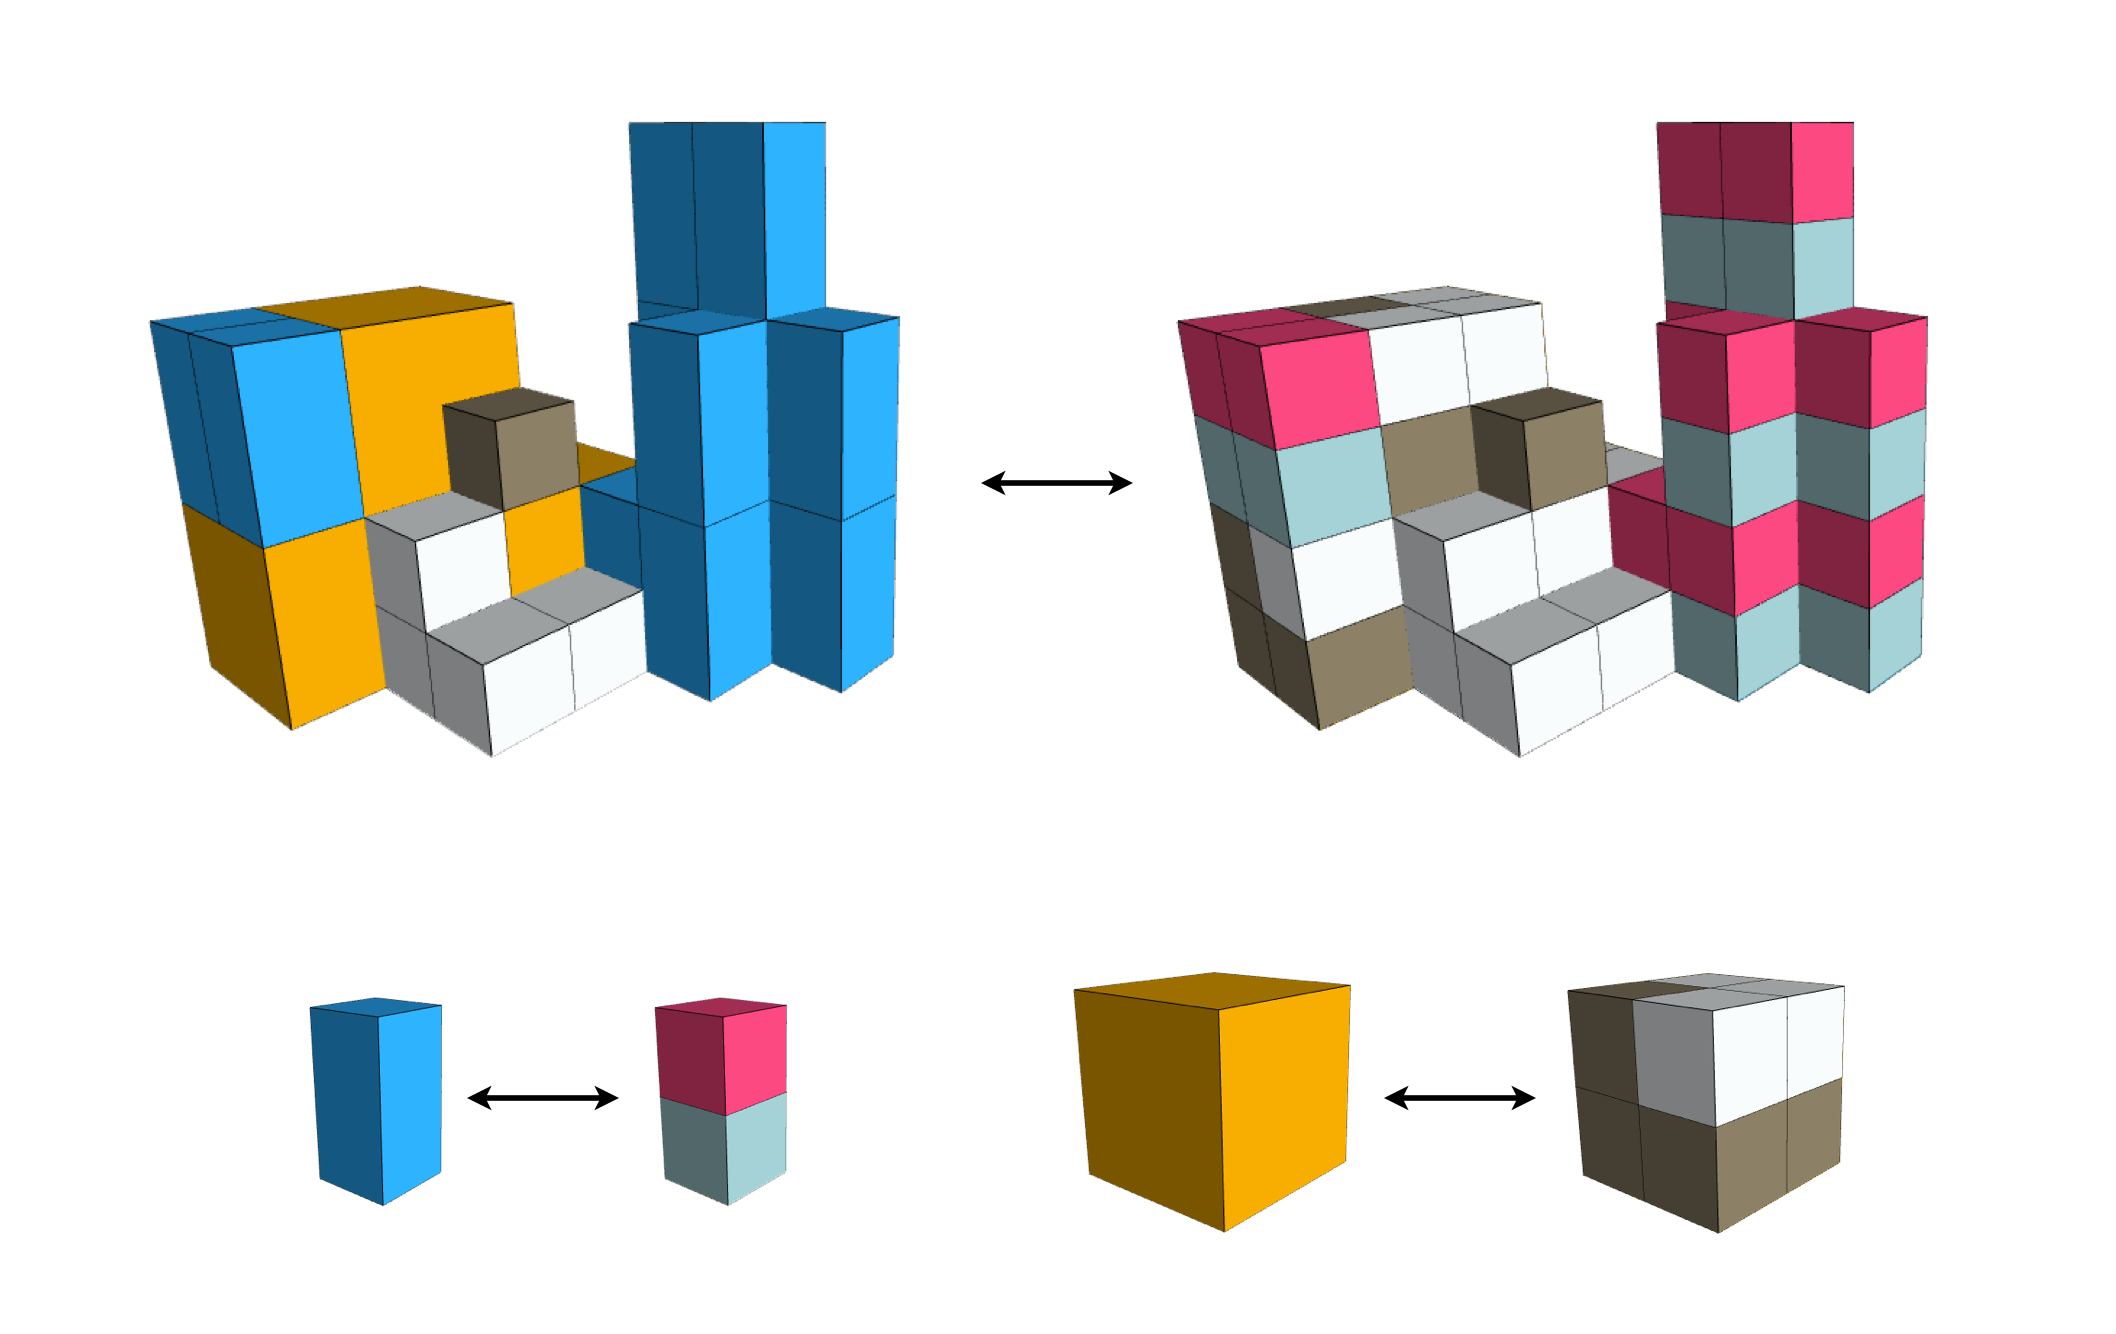
\includegraphics[width=\linewidth]{hierarchicalDecomp.png}
  \caption{Hierarchical decomposition of lattice assembly. All hierarchical components are parametrically linked to a hierarchical material definition.}
  \label{fig:hierarchicalDecomp}
\end{figure}

Borrowing some classes and frameworks I've started in DMDesign, I will create a new project for the work spawned from this thesis.  

%\begin{figure}
%  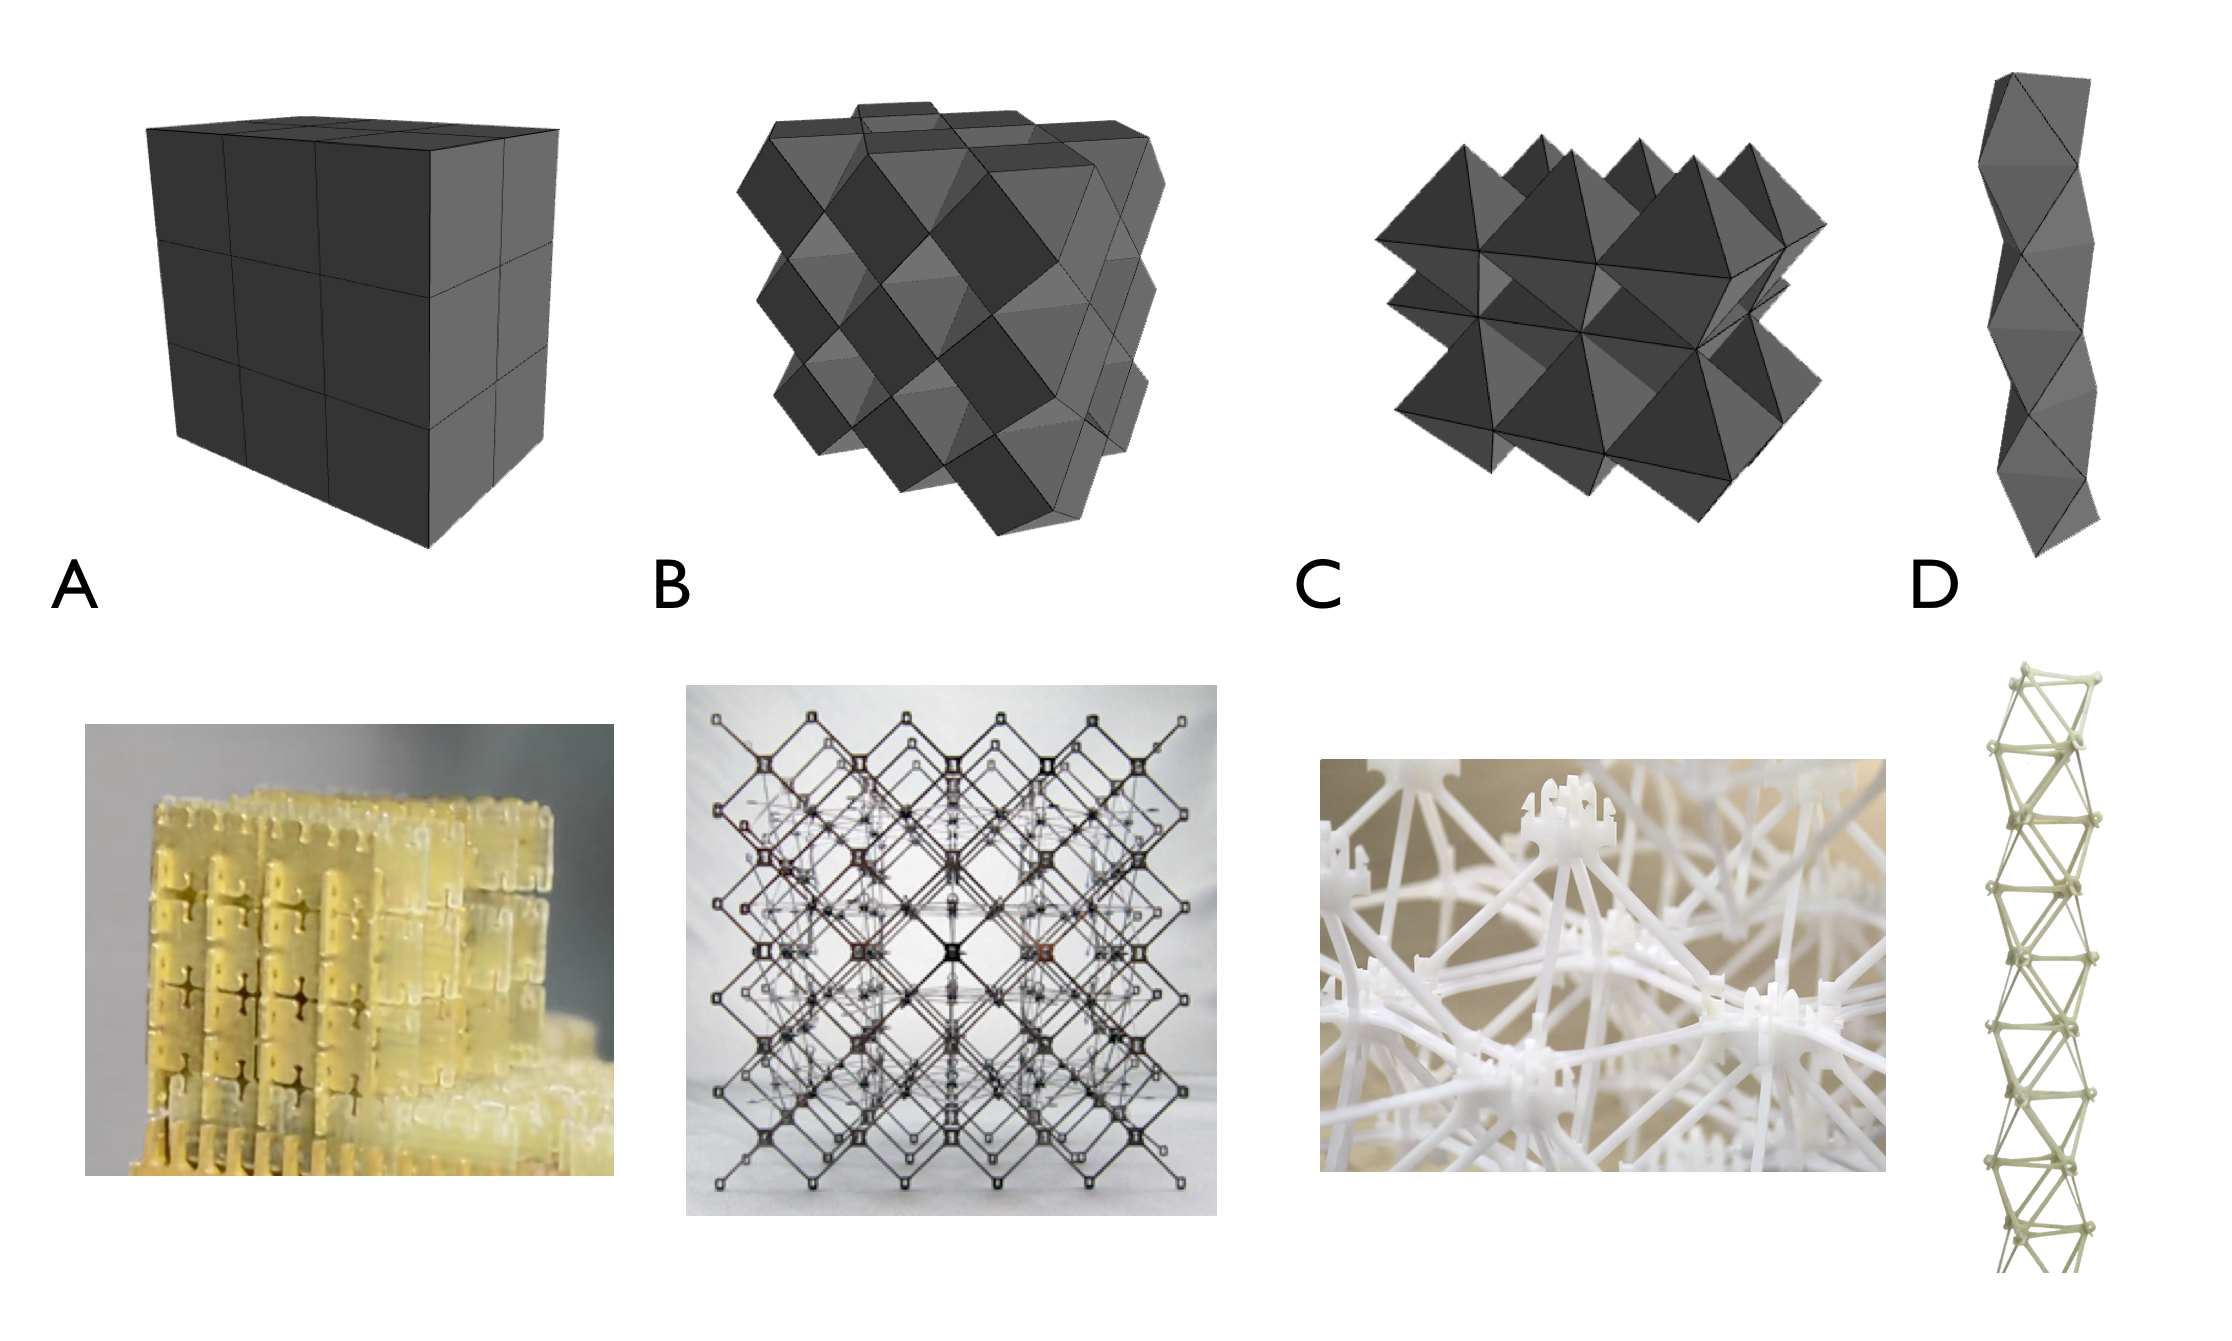
\includegraphics[width=\linewidth]{latticeVirtualRealComp.png}
%  \caption{Comparison of virtual lattice types with their real world counterparts.}
%  \label{fig: latticeVirtualRealComp}
%\end{figure}

%\begin{figure}
%  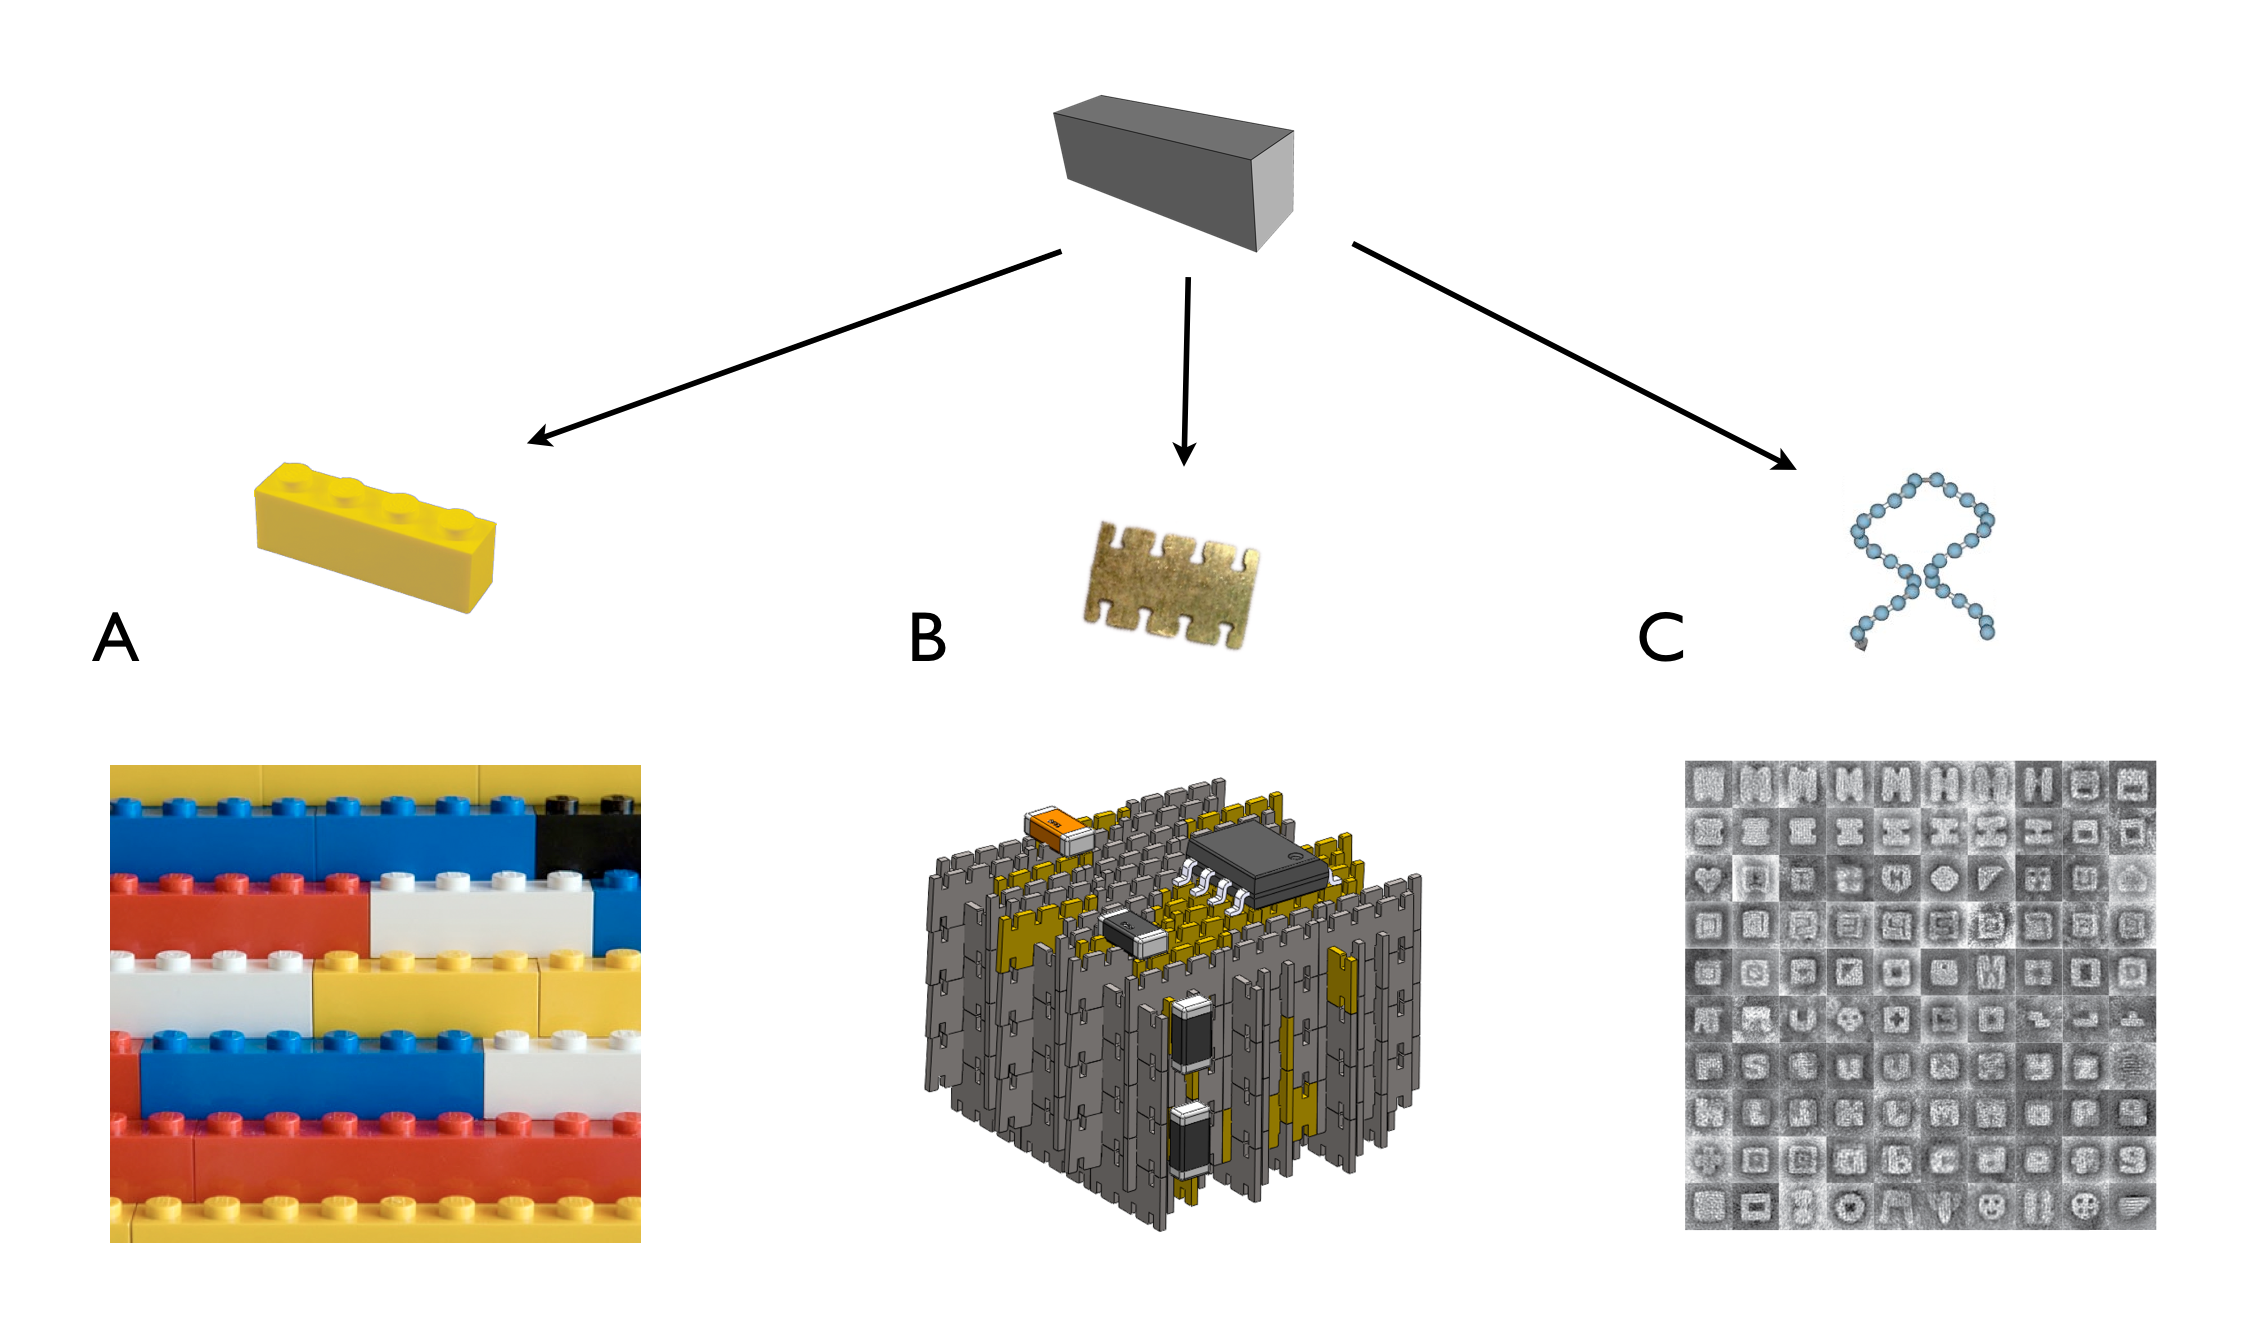
\includegraphics[width=\linewidth]{partAbstraction.png}
%  \caption{Part abstraction from lattice primitive.}
%  \label{fig: partAbstraction}
%\end{figure}

\subsection{Simulation}

The simulation portion of this project involves 
\\

I will need to implement some kind of collision detection for this system.  Due to the prevalence of gaming, there are an assortment of algorithms to speed up  collision detection over the obvious naive approaches.  Many physics engines rely on a boundary representation of an object to detect collision with other boundaries - if objects are moving too quickly this can lead to unexpected results.  The voxels in my geometry will together define a volume of space, and the cells forming the boundary of this volume are known; I will leverage this to cut down the computational costs of collision modeling in my simulations.

\subsection{Approach}

The proposed digital materials sandbox will be build in Javascript using the following dependencies (more may be added):
\begin{itemize}
\setlength\itemsep{0em}
\item \href{http://threejs.org/}{Three.js} is a library that makes WebGL easy to use without sacrificing much in performance
\item \href{http://requirejs.org/}{RequireJS} is a framework for asynchronously loading javascript modules and dependencies
\item \href{http://backbonejs.org/}{Backbone.js} is a framework for managing UI events and giving structure to an interactive application
\item \href{https://jquery.com/}{JQuery} is a library that simplifies interactions with HTML and helps maintain cross-browser support
\item \href{http://underscorejs.org/}{Underscore} is a library with lost of useful functions for dealing with arrays and javascript objects
\end{itemize}

I know I will take  performance hit writing this application in JavaScript as opposed to a strongly-typed language like C running natively, but I think for this first implementation it makes sense to do start with a programming environment that I can rapidly develop in and experiment.  If it turns out that I need to design very large structures or performance is getting in the way, I will consider porting the codebase into another language.  With some optimization of the rendering, it is possible to render 100-200k voxels on the screen at 30fps in Three.js.  
\\

Aside from my own comfort as a developer, I'm interested in using HTML5/Javascript for this application because it allows much easier access to the code than any other platform.  Though user studies are not a component of this work, there is a long history of communities of users building things in these types of sandbox environments that surpass anything the developers were able to imagine.  There is a lot of talent beyond the immediate neighborhood of CBA, and I'd like to try to make this codebase as available as possible for anyone interested in exploring this new way of making things.

%\subsection{Assembly}
%
%\begin{figure}
%  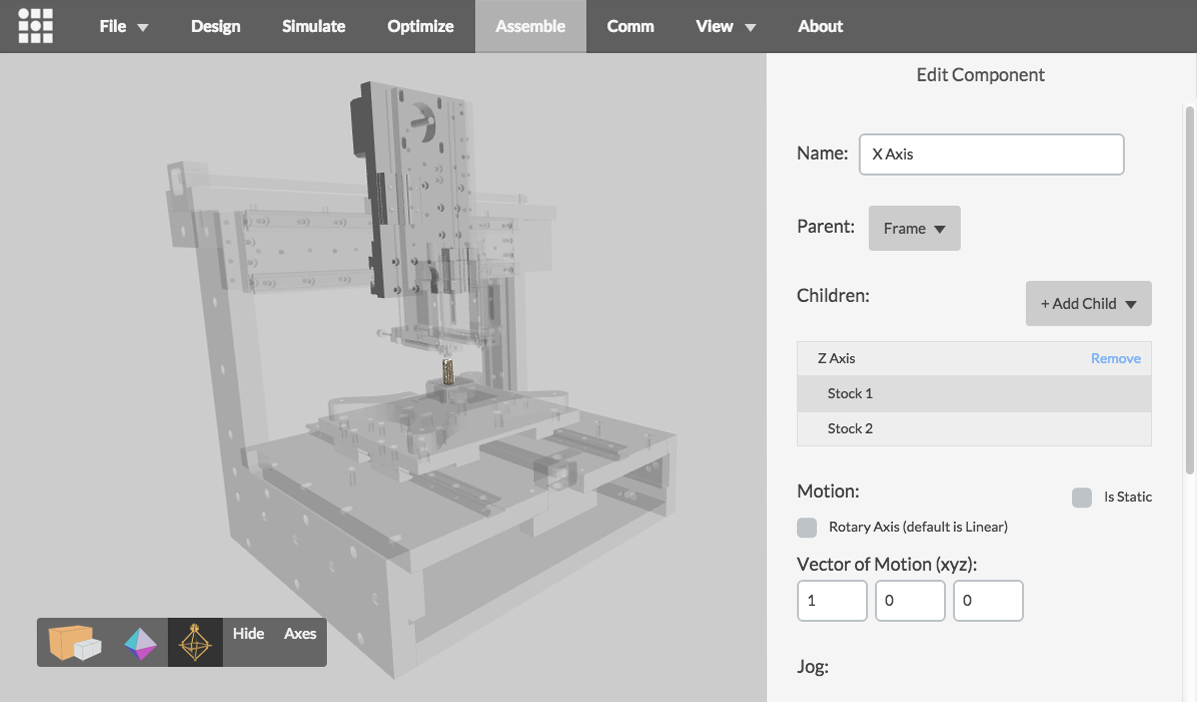
\includegraphics[width=\linewidth]{assemblerSetup1.png}
%  \caption{Screenshot of current assembler config GUI.}
%  \label{fig: assembleSetup1}
%\end{figure}
%
%\begin{figure}
%  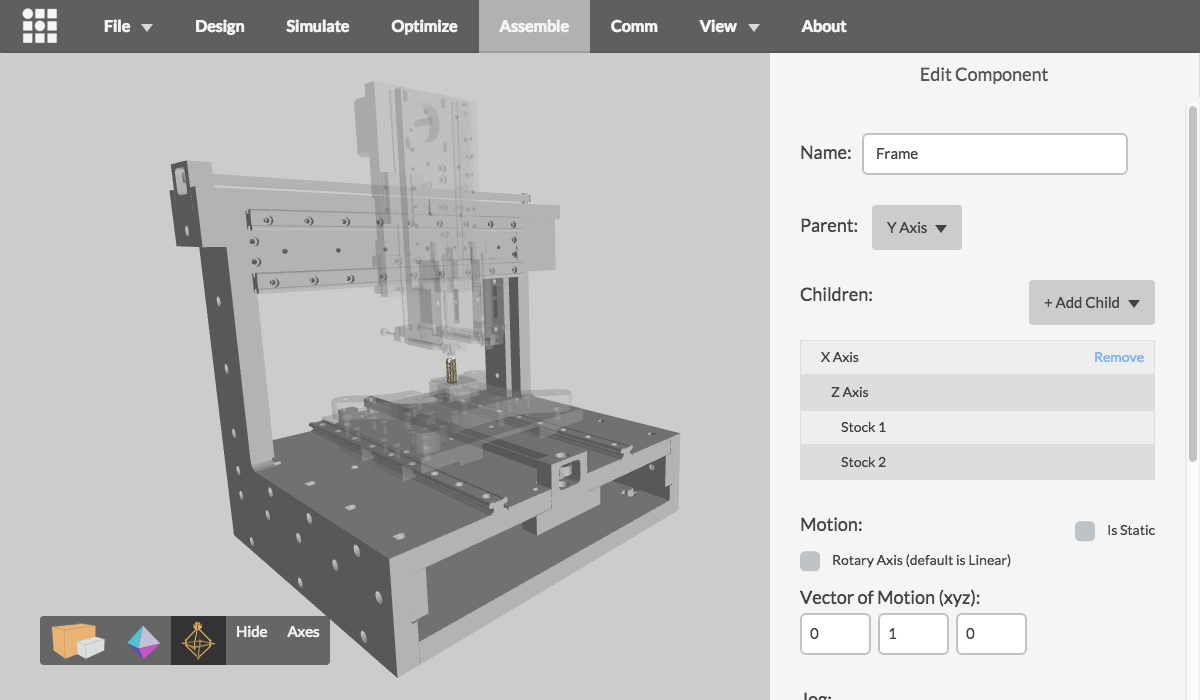
\includegraphics[width=\linewidth]{assemblerSetup2.png}
%  \caption{Screenshot of current assembler config GUI.}
%  \label{fig: assembleSetup2}
%\end{figure}
%
%urdf, tree description for abstraction
%calculate reverse kinematics
%abstraction of strategies and assemblers/low level operation

%\subsection{GUI}
%
%\begin{figure}
%  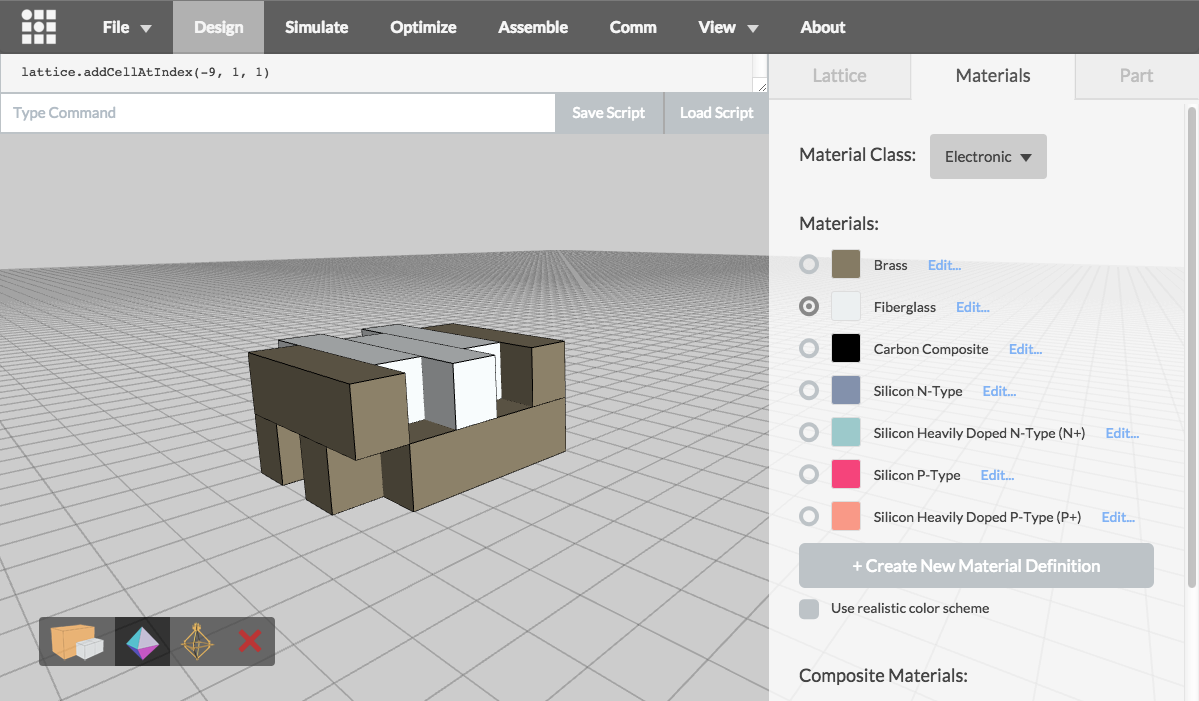
\includegraphics[width=\linewidth]{designGUI.png}
%  \caption{Screenshot of current design GUI.}
%  \label{fig: designGUI}
%\end{figure}
%
%\begin{figure}
%  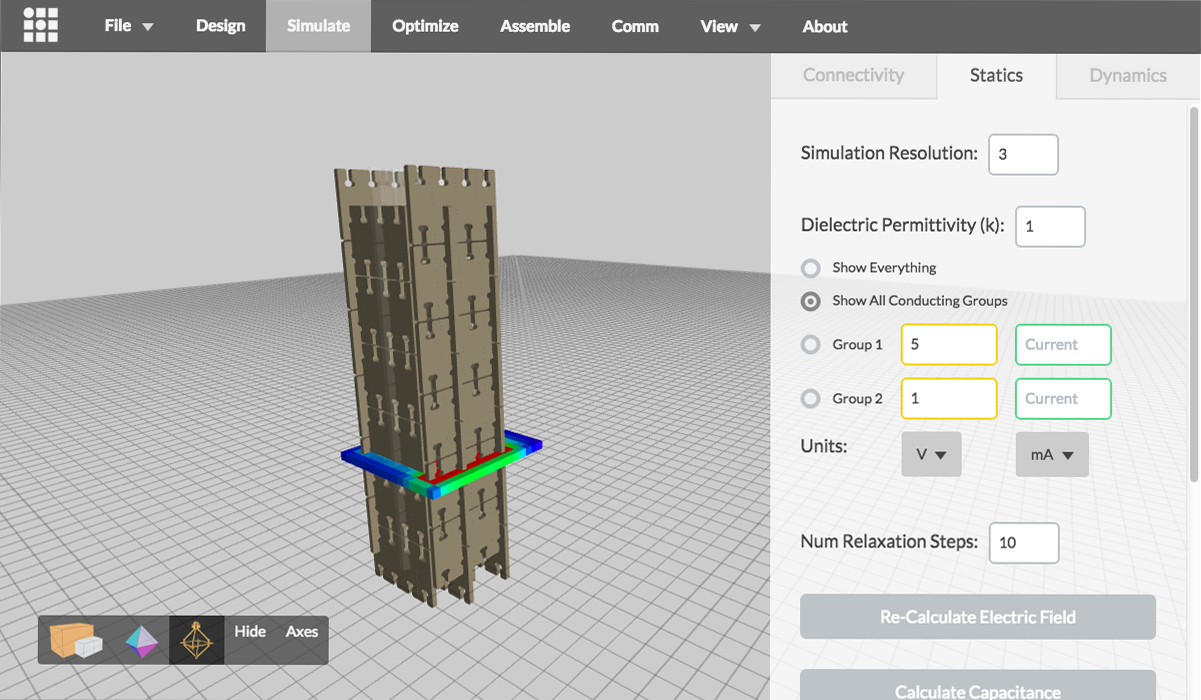
\includegraphics[width=\linewidth]{simGUI.png}
%  \caption{Screenshot of current simulation GUI.}
%  \label{fig: simGUI}
%\end{figure}
%
%\begin{figure}
%  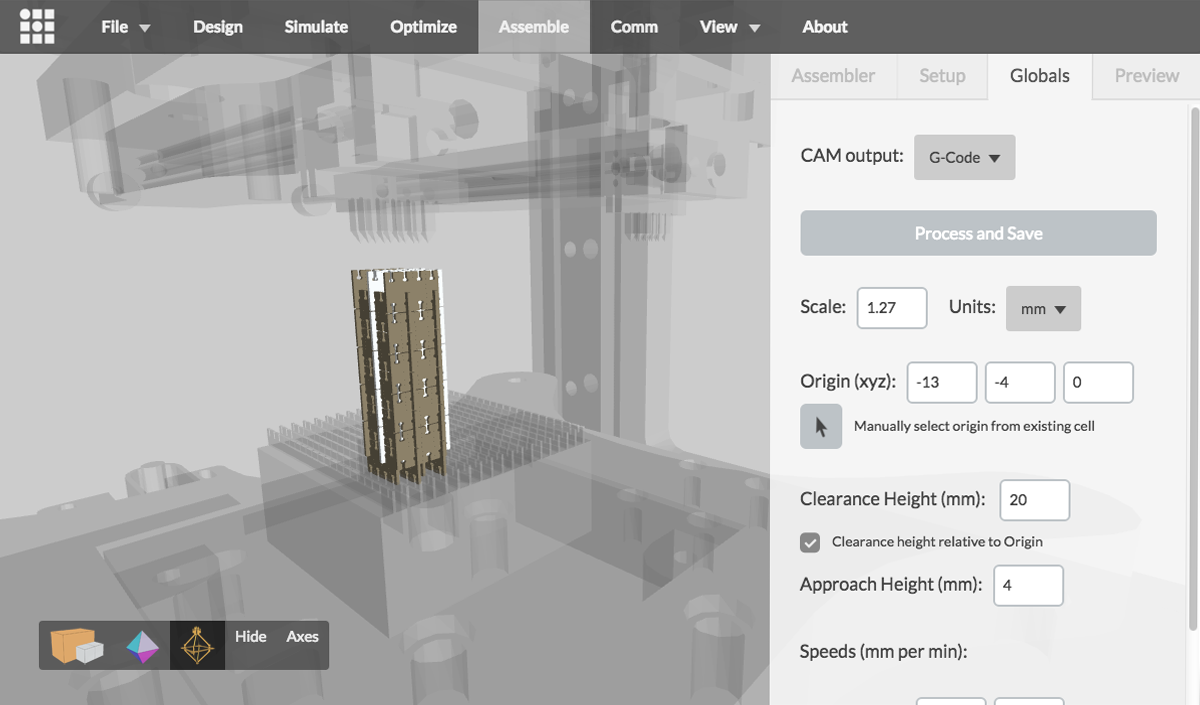
\includegraphics[width=\linewidth]{assembleGUI.png}
%  \caption{Screenshot of current assemble GUI.}
%  \label{fig: assembleGUI}
%\end{figure}
%
%javascript, etc, etc

%\subsection{API}
%
%Lattice, Cell, Material, CompositeMaterial classes.
%
%\begin{figure}
%  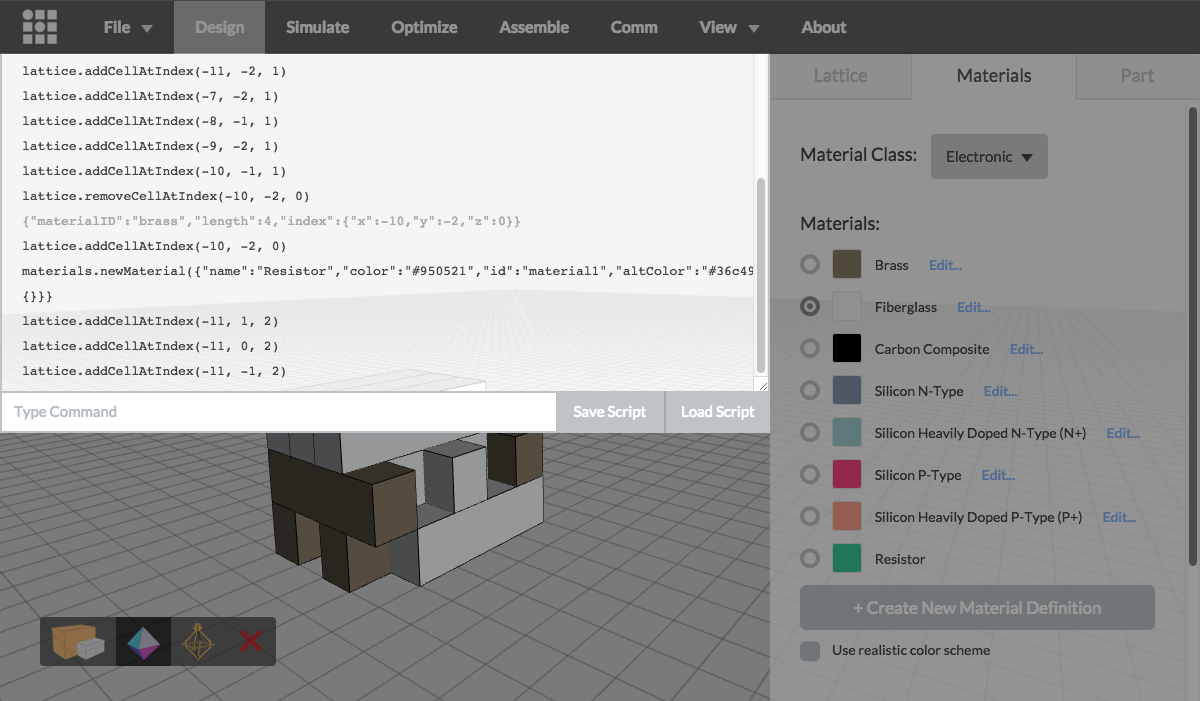
\includegraphics[width=\linewidth]{scriptGUI.png}
%  \caption{Screenshot of current script GUI for API with scripting console highlighted.}
%  \label{fig: scriptGUI}
%\end{figure}
%
%asdfdsf

\section{Contribution}

As outlined in previous sections, the main contribution of this work is to create a design/simulation environment where we can start to explore the rich design space around digital materials is a physically realistic way.
set up for optimization
wolfram quote

\section{Evaluation}

?????

\section{Resources Required}

The majority of the work involved in this thesis will happen in the computer and require no material resources.  If required, I will use CBA's cluster for highly parallel computational operations.  Fabrication of assemblers and parts to be used in the digital assembler workflows should be considered outside the scope of material resources required by this thesis, and will be supplied by CBA.

\section{Schedule}

\begin{description}
  \item[11/6/15]\tabto{1.5cm}Proposal Due
  \item[11/9/15]\tabto{1.5cm}Crit Day Presentation
  \item[11/15]\tabto{1.5cm}Design and assembly workflow for digital materials is in a working state.  I will use elements of the classes and framework developed in that project to begin a new project specifically for the completion of the thesis.  This new project will only be concerned with the design and simulation of multimaterial assemblies on a cubic lattice.
  \item[12/15]\tabto{1.5cm}
  \item[1/15]\tabto{1.5cm}I will spend January at NASA Ames to work with Kenny Cheung, Ben Jenett, and Daniel Cellucci on bringing in one of our new locomotion robots (Mojo) into my software workflow.  By this time I should have completed a refactor of the assembler tree code.  If successful, incorporating the new robot into my software will be accomplished entirely through the GUI, generating a config file that I can load into the codebase. 
  \item[2/15]\tabto{1.5cm}
  \item[3/15]\tabto{1.5cm}
  \item[4/15]\tabto{1.5cm}
  \item[5/15]\tabto{1.5cm}
  \item[6/6]\tabto{1.5cm}Thesis Due
\end{description}

}
